\documentclass[12pt,english]{article}

\usepackage{mathptmx}

\usepackage[section]{placeins}

\usepackage{color}

\usepackage[dvipsnames]{xcolor}

\definecolor{darkblue}{RGB}{0.,0.,139.}



\usepackage[top=1in, bottom=1in, left=1in, right=1in]{geometry}



\usepackage{amsmath}

\usepackage{amstext}

\usepackage{amssymb}

\usepackage{setspace}

\usepackage{lipsum}



\usepackage[authoryear]{natbib}

\usepackage{url}

\usepackage{booktabs}

\usepackage[flushleft]{threeparttable}

\usepackage{graphicx}

\usepackage[english]{babel}

\usepackage{pdflscape}

\usepackage[unicode=true,pdfusetitle, bookmarks=true,bookmarksnumbered=false,bookmarksopen=false, breaklinks=true,pdfborder={0 0 0},backref=false, colorlinks,citecolor=black,filecolor=black, linkcolor=black,urlcolor=black] {hyperref}

\usepackage[all]{hypcap} % Links point to top of image, builds on hyperref

\usepackage{breakurl}    % Allows urls to wrap, including hyperref



\linespread{2}



\begin{document}



\begin{singlespace}

\title{Utility-Scale Solar Site Suitability in Oklahoma\thanks{Many thanks to Dr. Tyler Ransom at the OU Economics Department for teaching me the professional skills necessary to be a competent economist, and to Dr. Aparna Mitra for still being the coolest human on Earth.}}

\end{singlespace}



\author{Alex Nongard\thanks{Department of Economics, University of Oklahoma.\
E-mail~address:~\href{mailto:nongard@ou.edu}{nongard@ou.edu}}}



% \date{\today}

\date{May 8, 2018}



\maketitle



\begin{abstract}

\begin{singlespace}

Multicriteria Decicion Analysis (MCDA) is a common technique used in Geographic Information Science (GIS), but so far has been rarely applied to economic questions, at least explicitly. We apply an MCDA to the problem of finding a suitable location for a utility-scale (1MW+) solar energy plant in the state of Oklahoma, concerned with land cover suitability, land slope, land cost, and solar irradiation. Our findings are roughly congruent with common knowledge, that Western Oklahoma would be most appropriate for siting a utility-scale solar energy farm. 

\end{singlespace}



\end{abstract}

\vfill{}





\pagebreak{}





\section{Introduction}\label{sec:intro}

Oklahoma is a very sunny and windy place. Estimates by the \citet{lopez} at the National Renewable Energy Laboratory (NREL) and the American Wind Energy \citet{awea} say that Oklahoma is 10th in overall potential for utility-scale solar photovoltaic energy production, and ninth for accessible wind energy resources. Despite these rankings, Oklahoma is actually ranked number two for installed wind capacity (just behind Texas) and 42nd for installed solar according to Solar Energy Industries \citet{seia}! Because of the untapped nature of solar in Oklahoma, especially compared to other renewables, there are a lot of opportunities for expansion in the future. This paper provides a preliminary analysis of suitable sites for utility-scale (1MW or greater) solar installations. We use Multicriteria Decision Analysis (MCDA) to assess data on solar irradiation (insolation), land gradient, land cover, and land cost to establish the most optimal areas for utility-scale solar farms within the state of Oklahoma. All statistical analyses were performed in R unless otherwise specified. 

\pagebreak{}

\section{Literature Review}\label{sec:litreview}

There are many different potential criteria to consider when choosing a location for a utility-scale solar farm. How far is the plant generating the energy from the people it will power? What is the cost of energy production going to be, relative to other types of energy? There are also more nebulous questions to answer, which are difficult to quantify without very explicit data. For instance, \citet{brewer} shows that using social acceptability data gathered from surveys, prime areas of potential solar development land are unacceptable to many citizens, such as in state parks or areas close to human development. Other criteria that are often considered: siting in areas that minimize biological impacts to some ecosystem (\citet{stoms}), human factors such as projected population, land need, and water usage growth (\citet{omitaomu}), and geopolitical factors such as availability of subsidies, politically unacceptable areas, and potential regulation (\citet{tisza}).  

As there are many different types of 'utility-scale solar power plant' (defined as a solar power plant that has at least 1MW production), we are not concerning ourselves with the individual specifications and needs of different types of plants (solar photovoltaic, concentrated solar power, etc.). We decided, for simplicity's sake and because of a lack of clear and available data, to only use some of the most universal and accessible physical and economic criteria for analysis. Therefore, we only account for insolation value, land gradient, land cover, and land cost. What follows is a detailed analysis of our study, data, methods, results, and conclusions surrounding the potential use of utility-scale solar farms in the state of Oklahoma.  

\pagebreak{}


\section{Data}\label{sec:data}

The study area we chose for this analysis is the entirety of the State of Oklahoma. While most of our data operate irrespective of political boundaries within the state, the one exception is median house value (used as a proxy for land value), which operates at the census block level.  

According to the Oklahoma Mesonet, a system of environmental sensors and research scientists, geographically and climatologically, Oklahoma is a Southern Great Plains state. There are a wide range of land covers from east to west. In the extreme northeast of the state, Oklahoma is part of the Ozark Plateau. Here it is comparatively moderate in temperature, precipitation, and volatility. Moving west, things get dryer, warmer, and more unstable. To the extreme west of the Panhandle, Oklahoma becomes part of the Black Mesa plateau, which is much dryer, colder, and at higher elevation. The south of the state is hotter, wetter, and more volatile overall in temperature and precipitation range (\citet{arndt}).  

When considering site suitability for a utility-scale solar farm, the operation of which may be affected by the general climate, volatility, and weather events of an area, these geographic factors are important to take into consideration. Out of convenience, only a handful of criteria are here considered. The data we chose to use were gathered from a variety of sources: daily solar irradiance data were gathered from the Oklahoma Mesonet for all 98 currently-active Mesonet data gathering points stretching from Jan 1, 1994 - Jan 1, 2018 (\citet{mesonet}), slope data were gathered from the United States Geological Survey from 2011 (\citet{ned}), land cover data were gathered from the USGS GAP/Landfire National Terrestrial Ecosystems dataset 2011 (\citet{landcover}), and land cost data for each census block were gathered from the US Census Bureau, from 2012-2016 estimates of the American Community Survey (\citet{census}). The geographical data uses the Geographic Coordinate System GCS North American 1983 using the North American Datum from 1983.  

\pagebreak{}

\section{Empirical Methods}\label{sec:methods}

The intent behind this paper is to establish a relative scale of the appropriateness of installing utility-scale solar farms in the state of Oklahoma. To do that, we used an MCDA that took as arguments various thresholds and hard criteria for suitability in the state. Once we established reasonable criteria from each data source, we used raster multiplication to create a final map of suitable locations.  

The criteria we established come in two kinds: Boolean hard criteria (1 if suitable, 0 if unsuitable) where only suitable values are taken on to the next level, and continuous soft criteria where values are plotted along the entire distribution. Boolean hard criteria are used for the USGS land slope data, wherein land with a slope of >3 percent is inappropriate for siting use, and the USGS land cover data wherein certain types of land cover are inappropriate for siting use. The continuous soft criteria are used for the solar irradiance values, because even areas of comparatively low solar irradiance might make economic sense for siting, and for land cost, because even areas of comparatively expensive land might be appropriate given some exogenous factor.  

First, daily solar irradiation values for the entire Mesonet system from 1994-2018 were collapsed into a single value for each of the 98 sites. This was done by averaging the values for each site and is appropriate because for a long-term investment in something as capital intensive as a solar farm the average value will be a good indicator of the 'solar return' on investing on the site. This does exclude the possibility of the solar irradiance changing over time, but to keep analysis simple, assuming this is an adequate snapshot of long-term irradiance will do. Once 98 point values for solar irradiation were established, we used the  Ordinary Kriging command from the package gstat to spatially interpolate solar irradiance values across the state of Oklahoma in a smooth gradient. This completed the first soft criteria with the full distribution of potential solar values across the state, and is seen in Figure 1.  

Kriging is a geostatistical technique that belongs to a Gaussian family of linear least square estimation algorithms. It is used to interpolate data across a field using nearby point observations in the estimates. 

Per the GIS \citet{wiki}: 

"The kriging estimator is given by a linear combination

$$\hat{Z}(x_0)=\sum_{i=1}^n w_i(x_0) Z(x_i)$$

of the observed values $z_i=Z(x_i)$ with weights  $w_i(x_0),\;i=1,\ldots,n$ chosen such that the variance (also called ''kriging variance'' or ''kriging error''):

$$\sigma^2_k(x_0):=\mathrm{Var}\left(\hat{Z}(x_0)-Z(x_0)\right)=\sum_{i=1}^n\sum_{j=1}^n w_i(x_0) w_j(x_0) c(x_i,x_j)
+ \mathrm{Var}\left(Z(x_0)\right)-2\sum_{i=1}^nw_i(x_0)c(x_i,x_0)$$

is minimized subject to the unbiasedness condition:
$$
\mathrm{E}[\hat{Z}(x)-Z(x)]=\sum_{i=1}^n w_i(x_0)\mu(x_i) - \mu(x_0) =0
$$

The ''kriging variance'' must not be confused with the variance
$$
\mathrm{Var}\left(\hat{Z}(x_0)\right)=\mathrm{Var}\left(\sum_{i=1}^n w_iZ(x_i)\right)=\sum_{i=1}^n\sum_{j=1}^n w_i w_j c(x_i,x_j)
$$
of the kriging predictor $\hat{Z}(x_0)$ itself."

This technique is the standard for interpolating values across a field in GIS and spatial statistics given individual point values. We use it here because for the quality of information that we have and the highly customizable nature of the kriging process through R packages, there are no significantly better estimators that we could use. 


Next, land slope values were calculated from a DEM of the state of Oklahoma from the USGS. The National Elevation Dataset contains data at a spatial resolution of 10m. We reclassified the entire map of Oklahoma to either 1 (suitable, slope less than or equal to 3 percent) or 0 (unsuitable, slope greater than 3 percent). These data were imported into ESRI ArcGIS and then exported as a .tif file for use in R. This can be seen in Figure 2.

After that, we used the USGS GAP land cover dataset to identify suitable land cover types in the State of Oklahoma. There are 88 types of land cover represented in the State of Oklahoma, from "West Gulf Coastal Plain Upland Longleaf Pine Forest and Woodland" to "Developed, High Intensity." All of these different types are subclasses of nine overarching land-use types, however: "Developed and Other Human Use," "Open Water," "Recently Disturbed or Modified," "Introduced and Semi Natural Vegetation," "Nonvascular and Sparse Vascular Rock Vegetation," "Agricultural and Developed Vegetation," "Desert and Semi-Desert," "Shrub and Herb Vegetation," and "Forest and Woodland." We reclassified the entire map of Oklahoma to either 1 (suitable, "Shrub and Herb Vegetation," "Desert and Semi-Desert," "Agricultural and Developed Vegetation," "Introduced and Semi Natural Vegetation," and "Nonvascular and Sparse Vascular Rock Vegetation") or 0 (unsuitable, all other classes). These data were imported into ESRI ArcGIS and then exported as a .tif file for use in R.  This can be seen in Figure 3. 

The final soft-criteria map was already pre-processed: the median value of homes in each US census block was used as a proxy of land value, because no comprehensive maps of land value exist or are easily accessible for the state of Oklahoma. These data were imported into ESRI ArcGIS and then exported as a .tif file for use in R. This can be seen in Figure 4

Note: We did lose some information overall in the processing of these maps because of their different data sources. In order to do the next piece of analysis (raster multiplication), all maps needed to be of the same resolution, extent, projection, and shape. Due to idiosyncrasies in the data sources, this is not always the case, and the land cover dataset was resampled to match the others. As a consequence, not all of the information is accurate, and there is no measure of data loss, but we believe the loss to be minimal. 

\pagebreak{}



\section{Research Findings}\label{sec:results}

Once all these criteria maps were established, we multiplied them together to create a final map of relative suitability for utility-scale solar installations in the state of Oklahoma. This can be seen in Figure 5. White portions of the map represent data values that failed the Boolean hard criteria; the color gradient in the key is self-explanatory beyond that. The absolute numbers, however, are meaningless – only the relative scale matters.  

These results show that solar site suitability generally increases east to west along a semi-smooth gradient. There are many areas that are classed out by various Boolean hard criteria, mostly in the eastern part of the state. The two largest contiguous areas that fail that criteria are around the cities of Tulsa and Oklahoma City. The areas with the highest suitability scores are in the far western panhandle and in the southwest of the state. Table 1 includes the top 10 counties by mean suitability rank – that is, the average of all values that passed the Boolean hard criteria, with the higher values being the most suitable. Areas that pass the Boolean hard criteria but are less suitable because of their soft criteria stand out near Oklahoma City, Tulsa, and Stillwater; this is mostly because of the land cost layer, as land values are higher near these cities. 

\pagebreak{}


\section{Conclusion}\label{sec:conclusion}

These results are roughly congruent with common knowledge – that western Oklahoma is sunnier, flatter, cheaper, and more consistent than the rest of the state. From the map (Figure 5) we can see that if we are to build a utility-scale solar farm in the state of Oklahoma, we are far better off doing it in the extreme west of the state than we are in the east. The eastern portion of the state has a large portion of land that failed the Boolean hard classification, as well as overall the lowest solar potential. Land near cities is too expensive to make economic sense, where land in the west is cheap, sunny, flat, and of appropriate type.  

This analysis is incomplete, in that there are many additional criteria that could be applied to create a map of suitable locations. As discussed earlier, there are many different types of solar power, from rooftop solar to concentrated solar power using molten salt. Each has its own unique requirements, and a general analysis like this one will never encompass all technologies. Other concerns that could/should be included in future analysis: weather volatility, weather damage potential (hail, severe storms, etc.), climate change, and population distribution, among other things.  

Limitations from the nature of the data analysis are also semi-major. R is actually not the greatest piece of software to use for advanced GIS applications, at least not as the author knows it. Data conversion and resampling did reduce the overall quality of the data, potentially leading to some confounding results. A better analysis tool would be ESRI ArcGIS or any other GIS-specific software, where inherent difficulties in modeling spatial data are better accounted for. It is also not quite as easy to make visually pleasing to the eye in R - other software comes with default visualizations that far surpass what is possible in R at the author's level of knowledge. To illustrate what the same analysis would produce in ArcGIS, please see Figure 6. 

In conclusion, according to our analysis, western Oklahoma has the highest relative suitability for solar energy in Oklahoma. Eastern Oklahoma is typically inappropriate or subpar for solar investment, according to these analyses. Future research could be done to expand this analysis and make it more specific to the different concerns of individual technologies.  



\vfill

\pagebreak{}

\begin{spacing}{1.0}

\bibliographystyle{jpe}

\bibliography{References.bib}

\addcontentsline{toc}{section}{References}

\end{spacing}



\vfill

\pagebreak{}

\clearpage



%========================================

% FIGURES AND TABLES 

%========================================

\section*{Figures and Tables}\label{sec:figTables}

\addcontentsline{toc}{section}{Figures and Tables}



%----------------------------------------

% Figure 1

%----------------------------------------

\begin{figure}[ht!]

\centering

\bigskip{}

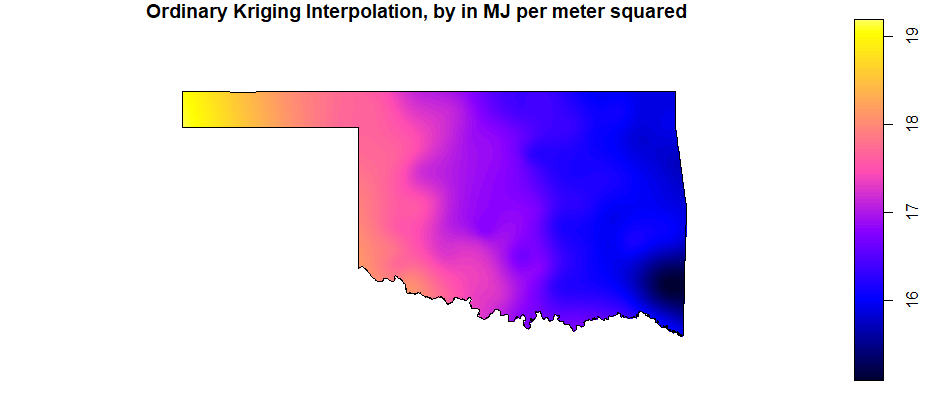
\includegraphics[width=.9\linewidth]{Rkrigf1.png}

\caption{Figure 1}

\label{fig:fig1}

\end{figure}

%----------------------------------------

% Figure 2

%----------------------------------------

\begin{figure}[ht!]

\centering

\bigskip{}

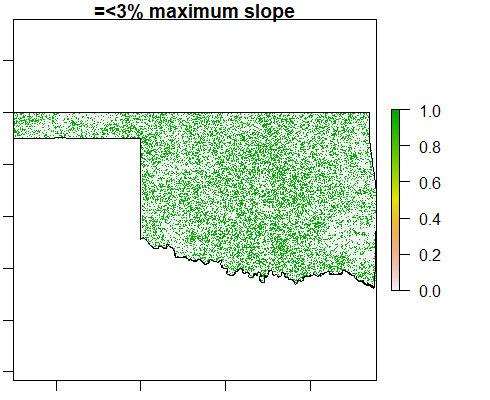
\includegraphics[width=.9\linewidth]{Rslope2.png}

\caption{Figure 2}

\label{fig:fig2}

\end{figure}

%----------------------------------------

% Figure 3

%----------------------------------------

\begin{figure}[ht!]

\centering

\bigskip{}

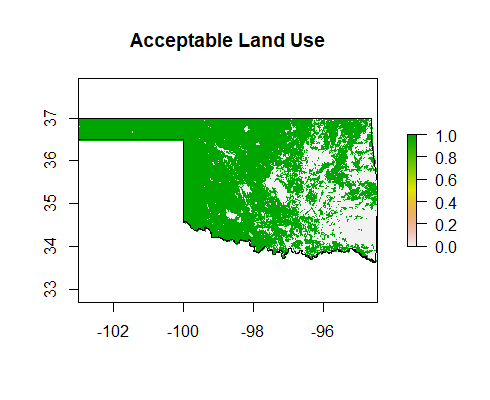
\includegraphics[width=.9\linewidth]{Rlanduse3.png}

\caption{Figure 3}

\label{fig:fig3}

\end{figure}

%----------------------------------------

% Figure 4

%----------------------------------------

\begin{figure}[ht!]

\centering

\bigskip{}

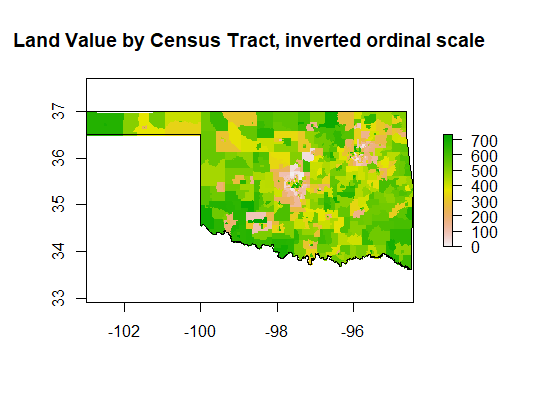
\includegraphics[width=.9\linewidth]{Rvalue4.png}

\caption{Figure 4}

\label{fig:fig4}

\end{figure}

%----------------------------------------

% Figure 5

%----------------------------------------

\begin{figure}[ht!]

\centering

\bigskip{}

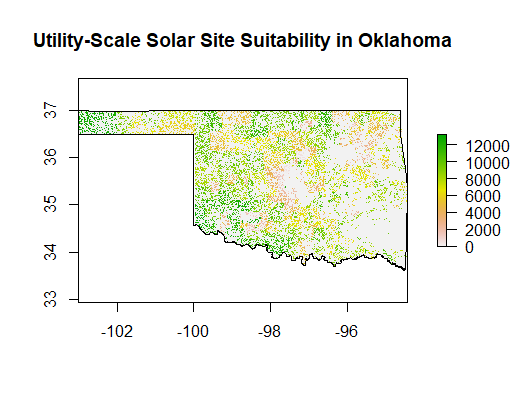
\includegraphics[width=.9\linewidth]{Rfinalplot.png}

\caption{Figure 5}

\label{fig:fig5}

\end{figure}


%----------------------------------------

% Figure 6

%----------------------------------------

\begin{figure}[ht!]

\centering

\bigskip{}

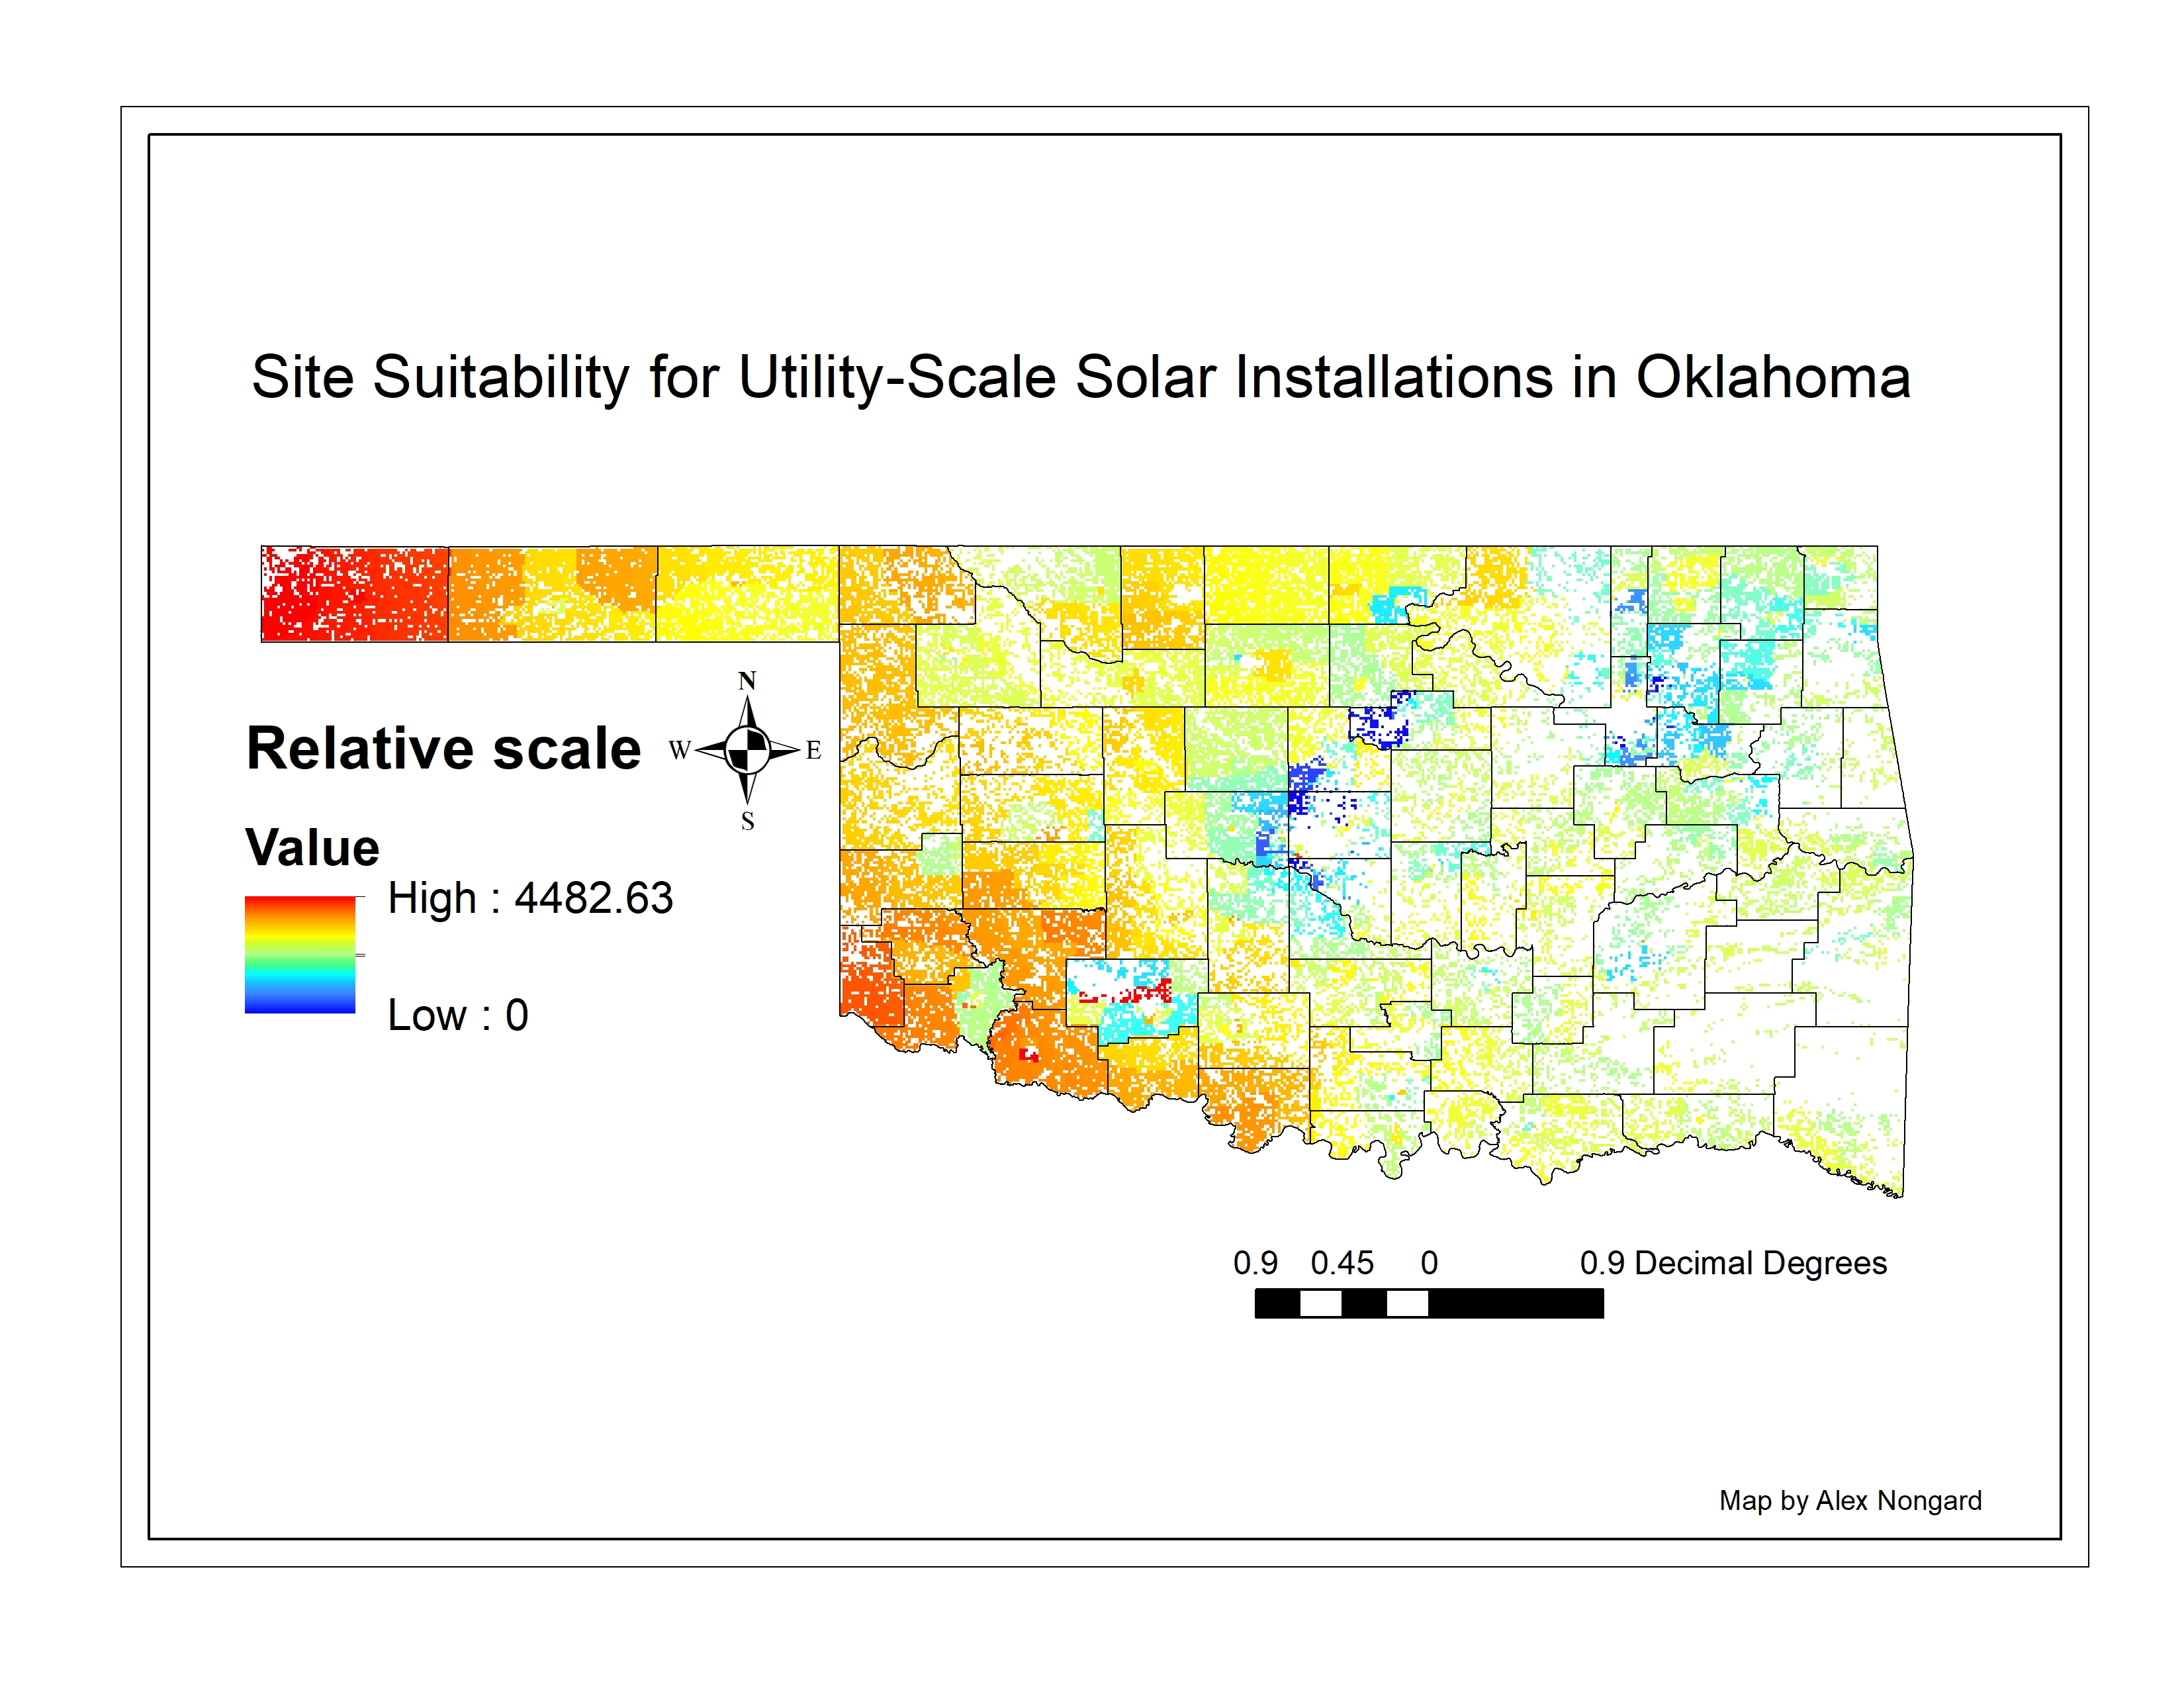
\includegraphics[width=.9\linewidth]{finalproject.jpg}

\caption{Final analysis produced in ESRI ArcGIS. White points indicate failed Boolean hard criteria.}

\label{fig:fig6}

\end{figure}

\FloatBarrier

%----------------------------------------

% Table 1

%----------------------------------------

% latex table generated in R 3.4.3 by xtable 1.8-2 package
% Mon May 07 15:23:29 2018
\begin{table}[bp!]
\caption{Top Ten Oklahoma Counties by Total Suitability Score}
\centering
\begin{tabular}{rlr}
  \hline
 & NAMELSAD & MEAN \\ 
  \hline
1 & Cimarron County & 3571.29 \\ 
  2 & Tillman County & 3423.32 \\ 
  3 & Texas County & 3297.42 \\ 
  4 & Harmon County & 3168.97 \\ 
  5 & Jackson County & 3122.11 \\ 
  6 & Kiowa County & 3090.70 \\ 
  7 & Grant County & 3081.97 \\ 
  8 & Cotton County & 3039.55 \\ 
  9 & Alfalfa County & 2921.85 \\ 
  10 & Greer County & 2838.94 \\ 
   \hline
\end{tabular}
\end{table}







\end{document}